%
% This document is licensed under the
%
%   Creative Commons Attribution-Noncommercial-Share Alike
%
% license. Please see LICENSE file for details.
%

\documentclass{InsightArticle}

\usepackage[dvipdfmx]{graphicx}
\usepackage{url}
\usepackage{textcomp}

\usepackage[dvipdfmx,
bookmarks,
bookmarksopen,
backref,
colorlinks,linkcolor={blue},citecolor={blue},urlcolor={blue},
]{hyperref}


\title{Unwarping Echo Planar Images Using CMTK\footnote{This document is licensed under
    the Creative Commons Attribution License Version 3.0.}}

\release{1.0}

\author{Torsten Rohlfing}
\authoraddress{Neuroscience Program, SRI International, Menlo Park, CA}

\begin{document}

\maketitle

\ifhtml
\chapter*{Front Matter\label{front}}
\fi


\begin{abstract}
\noindent This document describes the workflow for unwarping echo planar MR
images (EPI), in particular diffusion-weighted images, using an acquisition method
with reversed phase encoding and the tools of the Computational Morphometry
Toolkit (CMTK).
\end{abstract}

\tableofcontents

\clearpage
\section{Introduction}

\cite{HollKupeDale:2010}

\subsection{CMTK}

Unlike the previous two items, The Computational Morphometry Toolkit (CMTK) is
{\bf free}, and that's as in both free beer and free speech. CMTK is available
both in source code, licensed under the GPLv3, and as pre-compiled binary
distributions from \url{http://nitrc.org/projects/cmtk/}. If you are using
NeuroDebian, you can also install CMTK directly.

We shall assume that CMTK has been installed such that its tools can be run as
\begin{verbatim}
cmtk <tool> <arg1> <arg2> ...
\end{verbatim}

{\bf You will need CMTK release 2.2.4 or later.} Versions prior to 2.2.0 do not
  support EPI unwarping, and versions 2.2.0 through 2.2.3 contain a bug that
  prevented proper initialization of the deformation field.

\section{Step-by-Step}

\subsection{Imaging}

On your MR scanner of choice, you will need to implement an acquisition like
the one described in Ref.~\cite{HollKupeDale:2010}. In short, before the $b=0$
image of your favourite DWI acquisition sequence, you need to acquire an
additional $b=0$ image with phase-encoding direction reversed, thus resulting
in an image that is flipped in the phase-encoding direction and also distorted
by the ``opposite'' distortion field. 

{\bf Note that CMTK will not help you set up the acquisition - this is outside
the scope of the toolkit and also outside the scope of this manual.}

\begin{figure}[tbp]
\begin{center}
\begin{tabular}{cc}
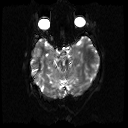
\includegraphics[width=.47\linewidth]{eps/b0_bwd} &
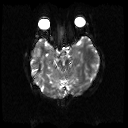
\includegraphics[width=.47\linewidth]{eps/b0_fwd} \\
(a) & (b) \\
\\
\end{tabular}
\begin{tabular}{ccc}
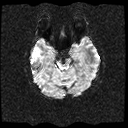
\includegraphics[width=.31\linewidth]{eps/b1} &
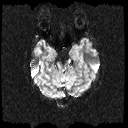
\includegraphics[width=.31\linewidth]{eps/b2} &
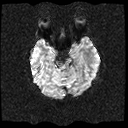
\includegraphics[width=.31\linewidth]{eps/b3} \\
(c) & (d) & (e) \\
\\
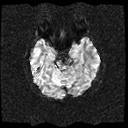
\includegraphics[width=.31\linewidth]{eps/b4} &
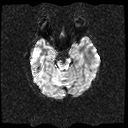
\includegraphics[width=.31\linewidth]{eps/b5} &
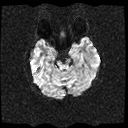
\includegraphics[width=.31\linewidth]{eps/b6} \\
(f) & (g) & (h) \\
\end{tabular}
\end{center}
\caption{(a) Axial slice from $b=0$ image acquired with reversed phase-encoding
  direction. (b) Aame slice from $b=0$ image acquired with standard
  phase-encoding direction. (c) through (h) Same slice from six different
  diffusion-weighted images acquired with standard phase-encoding direction.}
\label{fig:B0FwBw}
\end{figure}

\subsection{DICOM Image Stacking}

Assume that the DICOM files containing the EPI data are stored in the
``\texttt{dicom/}'' directory. These are stacked into 3D images in
NIFTI-format using the following CMTK command:
\begin{verbatim}
cmtk dcm2image -vx -O dwi/image\%d.nii dicom/
\end{verbatim}

This will result in a series of continuously numbered images in NIFTI format,
all stored in the <tt>dwi/</tt> directory.

Let us assume that we are using a 6-gradient-direction DWI setup with a single
reverse phase-encoded $b=0$ image acquired first, followed by the standard
$b=0$ image, followed by six diffusion images with different gradient
directions. In this case, we should find the following files:
\begin{description}
\item[\tt dwi/image1.nii] -- reverse phase-encoded $b=0$ image
\item[\tt dwi/image2.nii] -- standard phase-encoded $b=0$ image
\item[\tt dwi/image3.nii] -- 1st diffusion image
\item[\tt dwi/image4.nii] -- 2nd diffusion image
\item[\tt dwi/image5.nii] -- 3rd diffusion image
\item[\tt dwi/image6.nii] -- 4th diffusion image
\item[\tt dwi/image7.nii] -- 5th diffusion image
\item[\tt dwi/image8.nii] -- 6th diffusion image
\end{description}

\section{Concluding Remarks}

\section*{Acknowledgments}

\bibliographystyle{UnwarpEchoPlanar}
\bibliography{UnwarpEchoPlanar}

\clearpage
\appendix

\section{Example Data}

\end{document}

